\section{Exercise 1}

Hill's Surfaces:

\begin{equation}
    x^2 + Y^2 + \frac{2(1-\mu)}{r_1} + \frac{2 \mu}{r_2} = C
\end{equation}

\subsection*{a.}
The parameters in the above equations mean the following:
\begin{itemize}
    \item x,y: coordinates in the space-plane going through both large celestial bodies in the three-body problem. The origin is the barycenter of masses one and two.
    \item $\mu$: parameter of the restricted circular three-body problem, equal to $m_2$, the mass of body two.
    \item $r_1$: distance from body one to body three, which is equal to $\sqrt{(\mu+x)^2+y^2+z^2}$
    \item $r_2$: distance from body two to body three, which is equal to $\sqrt{(1-\mu-x)^2+y^2+z^2}$
    \item C: Jacobi's constant, integration constant from the equations of motion
\end{itemize}

The physical interpretation of Hill's surfaces is that they represent surfaces in space which can not be crossed by the third body.

\subsection*{b.}
Source picture: Wakker Figure 3.6 \\
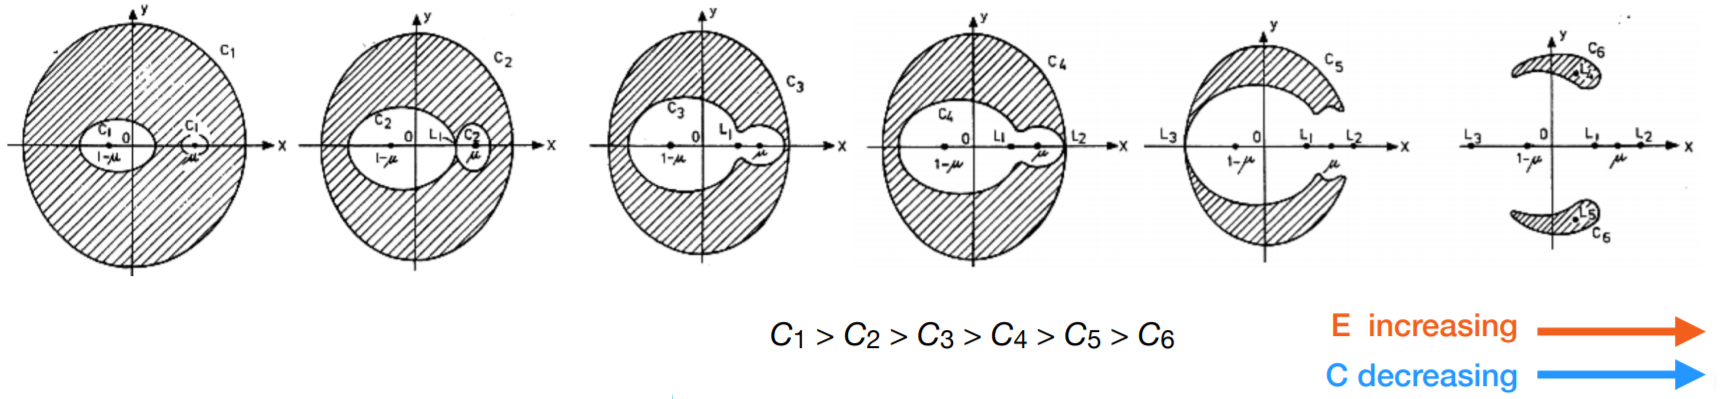
\includegraphics[scale = 0.5]{Chapters/Hill_Surfaces.png}

\subsection*{c.}
The physical meaning of the Lagrange libration points is that a third body on this point will maintain its relative position to the other two bodies; they are equilibrium points. The gravitational force, the centripetal force and the Coriolis force are all in balance in these points. While they are equilibrium points, there are alas not stable equilibrium points.

\subsection*{d.}
A Halo orbit is an orbit around Lagrangian libration points. Since the orbit is not naturally stable, it is called a slowly-changing elliptical orbit. A figure with the five Lagrangian points and their stability is shown below (credit: Wikipedia, Halo Orbit)\\
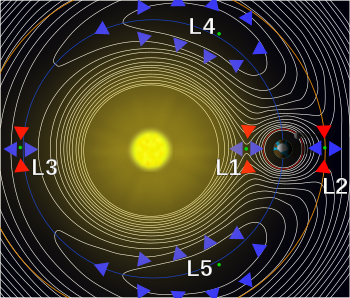
\includegraphics[scale = 1]{Chapters/Halo_Orbit.png} \\
Regarding the derivation of the stability: for L1, L2 and L3 there is a restoring force towards the central axis through masses one and two due to axis-symmetry, but for all other perturbation directions the Lagrangian points are unstable, since gravitational mass is only attracting and never repulsive.

\subsection*{e.}
Halo orbits are perfect for stable observations of space telescopes of a certain point in the celestial sky, or for deep-space observations without solar influence, or for solar observations while still being in permanent contact with the Earth. Similarly, Halo orbits are perfect for communication satellites for objects that are 'behind' the Sun or Moon, depending on which Lagrangian point is chosen.